% Options for packages loaded elsewhere
% Options for packages loaded elsewhere
\PassOptionsToPackage{unicode}{hyperref}
\PassOptionsToPackage{hyphens}{url}
\PassOptionsToPackage{dvipsnames,svgnames,x11names}{xcolor}
%
\documentclass[
  french,
  9pt,
  a4paper,
]{article}
\usepackage{xcolor}
\usepackage[top = 3cm,bottom = 2.5cm,left = 2.5cm,right =
2.5cm]{geometry}
\usepackage{amsmath,amssymb}
\setcounter{secnumdepth}{3}
\usepackage{iftex}
\ifPDFTeX
  \usepackage[T1]{fontenc}
  \usepackage[utf8]{inputenc}
  \usepackage{textcomp} % provide euro and other symbols
\else % if luatex or xetex
  \usepackage{unicode-math} % this also loads fontspec
  \defaultfontfeatures{Scale=MatchLowercase}
  \defaultfontfeatures[\rmfamily]{Ligatures=TeX,Scale=1}
\fi
\usepackage{lmodern}
\ifPDFTeX\else
  % xetex/luatex font selection
\fi
% Use upquote if available, for straight quotes in verbatim environments
\IfFileExists{upquote.sty}{\usepackage{upquote}}{}
\IfFileExists{microtype.sty}{% use microtype if available
  \usepackage[]{microtype}
  \UseMicrotypeSet[protrusion]{basicmath} % disable protrusion for tt fonts
}{}
\usepackage{setspace}
\makeatletter
\@ifundefined{KOMAClassName}{% if non-KOMA class
  \IfFileExists{parskip.sty}{%
    \usepackage{parskip}
  }{% else
    \setlength{\parindent}{0pt}
    \setlength{\parskip}{6pt plus 2pt minus 1pt}}
}{% if KOMA class
  \KOMAoptions{parskip=half}}
\makeatother
% Make \paragraph and \subparagraph free-standing
\makeatletter
\ifx\paragraph\undefined\else
  \let\oldparagraph\paragraph
  \renewcommand{\paragraph}{
    \@ifstar
      \xxxParagraphStar
      \xxxParagraphNoStar
  }
  \newcommand{\xxxParagraphStar}[1]{\oldparagraph*{#1}\mbox{}}
  \newcommand{\xxxParagraphNoStar}[1]{\oldparagraph{#1}\mbox{}}
\fi
\ifx\subparagraph\undefined\else
  \let\oldsubparagraph\subparagraph
  \renewcommand{\subparagraph}{
    \@ifstar
      \xxxSubParagraphStar
      \xxxSubParagraphNoStar
  }
  \newcommand{\xxxSubParagraphStar}[1]{\oldsubparagraph*{#1}\mbox{}}
  \newcommand{\xxxSubParagraphNoStar}[1]{\oldsubparagraph{#1}\mbox{}}
\fi
\makeatother


\usepackage{longtable,booktabs,array}
\usepackage{calc} % for calculating minipage widths
% Correct order of tables after \paragraph or \subparagraph
\usepackage{etoolbox}
\makeatletter
\patchcmd\longtable{\par}{\if@noskipsec\mbox{}\fi\par}{}{}
\makeatother
% Allow footnotes in longtable head/foot
\IfFileExists{footnotehyper.sty}{\usepackage{footnotehyper}}{\usepackage{footnote}}
\makesavenoteenv{longtable}
\usepackage{graphicx}
\makeatletter
\newsavebox\pandoc@box
\newcommand*\pandocbounded[1]{% scales image to fit in text height/width
  \sbox\pandoc@box{#1}%
  \Gscale@div\@tempa{\textheight}{\dimexpr\ht\pandoc@box+\dp\pandoc@box\relax}%
  \Gscale@div\@tempb{\linewidth}{\wd\pandoc@box}%
  \ifdim\@tempb\p@<\@tempa\p@\let\@tempa\@tempb\fi% select the smaller of both
  \ifdim\@tempa\p@<\p@\scalebox{\@tempa}{\usebox\pandoc@box}%
  \else\usebox{\pandoc@box}%
  \fi%
}
% Set default figure placement to htbp
\def\fps@figure{htbp}
\makeatother


% definitions for citeproc citations
\NewDocumentCommand\citeproctext{}{}
\NewDocumentCommand\citeproc{mm}{%
  \begingroup\def\citeproctext{#2}\cite{#1}\endgroup}
\makeatletter
 % allow citations to break across lines
 \let\@cite@ofmt\@firstofone
 % avoid brackets around text for \cite:
 \def\@biblabel#1{}
 \def\@cite#1#2{{#1\if@tempswa , #2\fi}}
\makeatother
\newlength{\cslhangindent}
\setlength{\cslhangindent}{1.5em}
\newlength{\csllabelwidth}
\setlength{\csllabelwidth}{3em}
\newenvironment{CSLReferences}[2] % #1 hanging-indent, #2 entry-spacing
 {\begin{list}{}{%
  \setlength{\itemindent}{0pt}
  \setlength{\leftmargin}{0pt}
  \setlength{\parsep}{0pt}
  % turn on hanging indent if param 1 is 1
  \ifodd #1
   \setlength{\leftmargin}{\cslhangindent}
   \setlength{\itemindent}{-1\cslhangindent}
  \fi
  % set entry spacing
  \setlength{\itemsep}{#2\baselineskip}}}
 {\end{list}}
\usepackage{calc}
\newcommand{\CSLBlock}[1]{\hfill\break\parbox[t]{\linewidth}{\strut\ignorespaces#1\strut}}
\newcommand{\CSLLeftMargin}[1]{\parbox[t]{\csllabelwidth}{\strut#1\strut}}
\newcommand{\CSLRightInline}[1]{\parbox[t]{\linewidth - \csllabelwidth}{\strut#1\strut}}
\newcommand{\CSLIndent}[1]{\hspace{\cslhangindent}#1}

\ifLuaTeX
\usepackage[bidi=basic]{babel}
\else
\usepackage[bidi=default]{babel}
\fi
% get rid of language-specific shorthands (see #6817):
\let\LanguageShortHands\languageshorthands
\def\languageshorthands#1{}


\setlength{\emergencystretch}{3em} % prevent overfull lines

\providecommand{\tightlist}{%
  \setlength{\itemsep}{0pt}\setlength{\parskip}{0pt}}



 


\usepackage{booktabs}
\usepackage{caption}
\usepackage{longtable}
\usepackage{colortbl}
\usepackage{array}
\usepackage{anyfontsize}
\usepackage{multirow}
\makeatletter
\@ifpackageloaded{float}{}{\usepackage{float}}
\floatstyle{plain}
\@ifundefined{c@chapter}{\newfloat{apptbl}{h}{lost}}{\newfloat{apptbl}{h}{lost}[chapter]}
\floatname{apptbl}{Tableau A}
\newcommand*\quartoapptblref[1]{Tableau \hyperref[#1]{A\ref{#1}}}
\@ifpackageloaded{caption}{}{\usepackage{caption}}
\DeclareCaptionLabelFormat{quartoapptblreflabelformat}{#1#2}
\captionsetup[apptbl]{labelformat=quartoapptblreflabelformat}
\newcommand*\listofapptbls{\listof{apptbl}{List of Tableaux annexess}}
\makeatother
\makeatletter
\@ifpackageloaded{float}{}{\usepackage{float}}
\floatstyle{plain}
\@ifundefined{c@chapter}{\newfloat{appfig}{h}{lost}}{\newfloat{appfig}{h}{lost}[chapter]}
\floatname{appfig}{Graphique A}
\newcommand*\quartoappfigref[1]{Graphique \hyperref[#1]{A\ref{#1}}}
\@ifpackageloaded{caption}{}{\usepackage{caption}}
\DeclareCaptionLabelFormat{quartoappfigreflabelformat}{#1#2}
\captionsetup[appfig]{labelformat=quartoappfigreflabelformat}
\newcommand*\listofappfigs{\listof{appfig}{List of Graphiques annexess}}
\makeatother
\makeatletter
\@ifpackageloaded{tcolorbox}{}{\usepackage[skins,breakable]{tcolorbox}}
\@ifpackageloaded{fontawesome5}{}{\usepackage{fontawesome5}}
\definecolor{quarto-callout-color}{HTML}{909090}
\definecolor{quarto-callout-note-color}{HTML}{0758E5}
\definecolor{quarto-callout-important-color}{HTML}{CC1914}
\definecolor{quarto-callout-warning-color}{HTML}{EB9113}
\definecolor{quarto-callout-tip-color}{HTML}{00A047}
\definecolor{quarto-callout-caution-color}{HTML}{FC5300}
\definecolor{quarto-callout-color-frame}{HTML}{acacac}
\definecolor{quarto-callout-note-color-frame}{HTML}{4582ec}
\definecolor{quarto-callout-important-color-frame}{HTML}{d9534f}
\definecolor{quarto-callout-warning-color-frame}{HTML}{f0ad4e}
\definecolor{quarto-callout-tip-color-frame}{HTML}{02b875}
\definecolor{quarto-callout-caution-color-frame}{HTML}{fd7e14}
\makeatother
\makeatletter
\@ifpackageloaded{caption}{}{\usepackage{caption}}
\AtBeginDocument{%
\ifdefined\contentsname
  \renewcommand*\contentsname{Table des matières}
\else
  \newcommand\contentsname{Table des matières}
\fi
\ifdefined\listfigurename
  \renewcommand*\listfigurename{Graphiques}
\else
  \newcommand\listfigurename{Graphiques}
\fi
\ifdefined\listtablename
  \renewcommand*\listtablename{Tableaux}
\else
  \newcommand\listtablename{Tableaux}
\fi
\ifdefined\figurename
  \renewcommand*\figurename{Graphique}
\else
  \newcommand\figurename{Graphique}
\fi
\ifdefined\tablename
  \renewcommand*\tablename{Tableau}
\else
  \newcommand\tablename{Tableau}
\fi
}
\@ifpackageloaded{float}{}{\usepackage{float}}
\floatstyle{ruled}
\@ifundefined{c@chapter}{\newfloat{codelisting}{h}{lop}}{\newfloat{codelisting}{h}{lop}[chapter]}
\floatname{codelisting}{Listing}
\newcommand*\listoflistings{\listof{codelisting}{Liste des Listings}}
\makeatother
\makeatletter
\makeatother
\makeatletter
\@ifpackageloaded{caption}{}{\usepackage{caption}}
\@ifpackageloaded{subcaption}{}{\usepackage{subcaption}}
\makeatother
\makeatletter
\@ifpackageloaded{fontawesome5}{}{\usepackage{fontawesome5}}
\makeatother
\newcounter{quartocallouttipno}
\newcommand{\quartocallouttip}[1]{\refstepcounter{quartocallouttipno}\label{#1}}
\usepackage{bookmark}
\IfFileExists{xurl.sty}{\usepackage{xurl}}{} % add URL line breaks if available
\urlstyle{same}
\hypersetup{
  pdftitle={Une part des salaires dans la VA élévée en 2025 en France},
  pdfauthor={Xavier Timbeau},
  pdflang={fr},
  colorlinks=true,
  linkcolor={blue},
  filecolor={Maroon},
  citecolor={Blue},
  urlcolor={Blue},
  pdfcreator={LaTeX via pandoc}}


%%% title.tex we use to call other packages. Because this works
\usepackage{titlepic}
\usepackage{titling}
\usepackage{graphicx}
\usepackage{fontspec}
\usepackage{placeins}
\usepackage{graphbox}
\usepackage{tikz}
\usepackage{geometry}
\usepackage{xcolor}
\usepackage{amsmath}
\usepackage[some]{background}
\usepackage{lipsum}
\usepackage{caption}
\usepackage{datetime}
\usepackage{xstring}
\usepackage{blindtext}
\usepackage{scrlayer-scrpage}

\setmainfont{OpenSans}[
  UprightFont = {*-Regular},
  BoldFont = {*-Bold},
  BoldItalicFont = {*-BoldItalic},
  ItalicFont = {*-Italic},
  Path = {_extensions/ofce/wp/OpenSans/},
  Extension = {.ttf}
]
\setsansfont{OpenSans}[
  UprightFont = {*-Regular},
  BoldFont = {*-Bold},
  BoldItalicFont = {*-BoldItalic},
  ItalicFont = {*-Italic},
  Path = {_extensions/ofce/wp/OpenSans/},
  Extension = {.ttf}
]

\def\getYear#1{\StrLeft{#1}{4}}
\def\getMonth#1{\StrMid{#1}{6}{7}}
\def\getDay#1{\StrRight{#1}{2}}

\def\jolimois#1{\monthname{\getMonth{#1}}}

\definecolor{quarto-callout-color}{HTML}{eeeeee}
\definecolor{quarto-callout-tip-color}{HTML}{dddddd}
\definecolor{quarto-callout-tip-color-frame}{HTML}{eeeeee}

\clearpairofpagestyles

\KOMAoptions{headsepline=true}

\pagestyle{scrheadings}
\setkomafont{pageheadfoot}{\small}

\rehead{Document de travail n°2025-23}
\lohead{\includegraphics[height=0.25cm]{\_extensions/ofce/wp/ofce\_m.png}}

\lofoot*{\thepage}
\refoot*{\thepage}
\begin{document}



\definecolor{ofcepbbleu}{RGB}{1, 97, 131}
\definecolor{ofcerouge}{RGB}{198, 45, 43}
\definecolor{scporouge}{RGB}{231, 0, 26}

\begin{titlepage}
  \backgroundsetup{
    scale=1,
    angle=0,
    opacity=1,
    contents={
  \begin{tikzpicture}[remember picture,overlay]
    \useasboundingbox (0,0) rectangle(\the\paperwidth,\the\paperheight);
      \node [anchor = center] at (-2.875-5.25,12.5) {\includegraphics[width=2.5cm]{\_extensions/ofce/wp/ofce\_m.png}};
      \node [anchor = center] at (-2.875-5.25,-12.75){\includegraphics[width=2.5cm]{\_extensions/ofce/wp/sciencespo.png}};
      \node [anchor = east] at (8.5,-11.5){\textcolor{black}{Publié le : 24
octobre 2025}};
      \node [anchor = east] at (8.5,-12){\textcolor{black}{Modifié le : 20
novembre 2025}};
      \node [anchor = east] at (8.5,13-0.7){\textcolor{gray}{\Huge\textit{Working Paper}}};
      \draw [thick,black](-5.75,-13) -- (-5.75,13);
      \draw [color = white, fill=ofcepbbleu] (8.7,11.4) rectangle (10.45,13.15);
      \draw [color = white, fill=ofcepbbleu, very thick] (8.75-.5,11.25-.5) rectangle (8.75+.6,11.25+.6);
      \node [anchor = east] at (11-0.7,13-0.7){\textcolor{white}{\huge\textbf{23}}};
      \node [anchor = east] at (10-0.74,12-0.67){\textcolor{white}{\textbf{2025}}};
    \end{tikzpicture}
  }
}
\BgThispage

\hspace{4cm}
\begin{minipage}{12.5cm}
  \vspace{5cm}
  \begin{flushleft}
    \begin{spacing}{2.5}
      \textcolor{scporouge}{\Huge\textbf{\textsf{Une part des salaires
dans la VA élévée en 2025 en France}}}
    \end{spacing}
   \vspace{5mm}
  \textcolor{scporouge}{\large\textbf{\textsf{Comparaisons
internationales de 30~ans de partage de la valeur ajoutée}}}
 \vspace{5mm}
    \vspace{20mm}
  \end{flushleft}

  
   \textbf{Xavier Timbeau},           OFCE, Sciences Po Paris
   
  % by-author
 \end{minipage}


%%
%% deuxieme page
\newpage
\pagestyle{empty}
\raisebox{-22cm}{
    \begin{minipage}[b]{40em}
      \textcolor{scporouge}{
        \textbf{CONTACT}}{

          \vspace{0.2cm}
          \vspace{0.2cm}

        \textbf{OFCE}

        10 place de Catalogne

        75014 Paris, FRANCE

        Tel : +33 1 44 18 54 24

        \url{https://www.ofce.sciences-po.fr}
      }
    \end{minipage}
}
%%
%%
\newpage
%% troisieme page
\pagestyle{empty}
%%  \raisebox{3cm}{\begin{minipage}{\linewidth}
%%  \includegraphics[width=2cm]{\_extensions/ofce/wp/ofce\_m.png}
%%
%%  \includegraphics[width=2cm]{\_extensions/ofce/wp/sciencespo.png}
%%  \end{minipage}}
%%

\LARGE\textbf{Une part des salaires dans la VA élévée en 2025 en France}

\large\textbf{Comparaisons internationales de 30~ans de partage de la
valeur ajoutée}

\vspace{1cm}


\par\rule{\textwidth}{0.5pt}

On explore différentes façons de calculer la notion de part des salaires
dans la valeur ajoutée. Le concept privilégié est celui de la part des
salaires \emph{corrigés de la non salarisation} dans la valeur ajoutée
\emph{nette de la consommation de capital fixe} des branches
\emph{marchandes hors services immobiliers}. Il peut être calculé pour
les pays européens. Il fait apparaître une position singulière de la
France où la part des salaires est plus élevé et s'est accrue de façon
importante. Bien que plus fragile empiriquement, le calcul de rendement
net d'impôts du capital productif confirme ce diagnostic
particulièrement préoccupant pour le tissu productif français.
L'ensemble des éléments présentés est reproductible à partir des codes
fournis.

\par\rule{\textwidth}{0.5pt}


\vspace{1cm}


version en ligne à https://xtimbeau.github.io/travail/


\vspace{1cm}

\begin{flushright}
   \linespread{1}\small{\textbf{Xavier
Timbeau}}, {\small{xavier.timbeau@sciencespo.fr}}\par
 % by-author
\end{flushright}
\vspace{2.5cm}
\begin{minipage}[b]{40em}
  \textcolor{scporouge}{
    \textbf{Remerciements}}{

      \vspace{0.2cm}
      \vspace{0.2cm}

    \textit{\small{Je remercie chaleureusement Elliot Aurissergues,
François Geerolf et Eric Heyer pour leurs remarques pertinentes et
stimulantes. Elles m'ont amené à aller plus loin dans les concepts et
les données. La confusion qui en découle est de ma seule
responsabilité.}}
  }
\end{minipage}
\end{titlepage}

%%% Define custom colors
% tip
\definecolor{quarto-callout-tip-color}{HTML}{000000}
\definecolor{quarto-callout-tip-color-frame}{HTML}{EEEEEE}

\vspace{2.5cm}

\renewcommand*\contentsname{Table des matières}
{
\hypersetup{linkcolor=}
\setcounter{tocdepth}{1}
\tableofcontents
}

\vspace{5cm}
\setstretch{1.25}
\section{Du partage de la VA au partage des
richesses}\label{du-partage-de-la-va-au-partage-des-richesses}

L'analyse du partage de la valeur ajoutée (graphique~\ref{fig-psal}) est
au cœur des débats sur la redistribution des richesses (voir notamment
Hurlin et Portier (1996), Timbeau (2002), Cotis (2009), Husson (2010),
Askenazy, Cette et Sylvain (2012), Piton (2019), Pak, Pionnier et
Schwellnus (2019), Cette, Koehl et Philippon (2019), Timbeau (2025),
Gendre et Thommen (2025)). Un indicateur souvent retenu est celui de la
part des salaires dans la valeur ajoutée. Nous discutons ici de la
construction de cet indicateur et de sa comparabilité entre pays.

\begin{figure}[htb]

\caption{\label{fig-psal}Part des salaires dans la VA nette}

\centering{

\subcaption{\label{fig-psal-1}Part des salaires dans la VA nette hors
services immobiliers (-L)}

\centering{

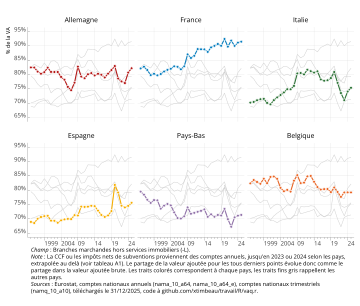
\includegraphics[width=1\linewidth,height=\textheight,keepaspectratio]{index_files/mediabag/index_files/figure-pdf/fig-psal-1-1.pdf}

}

}

\end{figure}%

\subsection{Du bon concept de part des
salaires}\label{du-bon-concept-de-part-des-salaires}

Trois points sont importants pour disposer du bon concept (voir Reis
(2022) pour une discussion et une revue de littérature sur ce point)\,:

\begin{itemize}
\tightlist
\item
  \textbf{Corriger des non salariés et leur imputer une masse
  salariale}. La correction habituelle consiste à affecter aux non
  salariés le même salaire que les salariés (généralement de la même
  branche)\,; c'est ainsi que traitent la question Cette, Koehl et
  Philippon (2019) et Gendre et Thommen (2025). Nous procédons à cette
  correction (appelée \emph{correction par les effectifs}) aux 21
  branches de la NACE rev. 2 niveau 1. Nous proposons une alternative en
  utilisant la mesure du revenu mixte (dite \emph{correction par le
  revenu mixte}), parce que l'affectation d'un salarie égal aux non
  salariés et aux salariés par branches conduit à imputer un équivalent
  masse salariale supérieur au revenu mixte des non salariés{[}\^{}1{]}.
  En France, le revenu mixte (des non-salariés) est passé de 30\% de la
  masse salariale (autant pour le ratio des effectifs) au début des
  années 1970 à un peu moins de 10\% (presque 15\% pour les effectifs)
  en 2024. Malheureusement, le revenu mixte par branche n'est pas
  diffusé systématiquement par les Etats membres de l'UE. Ces
  corrections modifient significativement la part des salaires dans la
  valeur ajoutée, suivant la méthode, parce que non seulement la part
  des non salariés et de leur revenu mixte varie dans le temps, de façon
  différente par un effet de structure (moins d'agriculteurs) et de
  nature (les non salariés sont moins rémunérés aujourd'hui), de façon
  différente par pays (graphique~\ref{fig-psal} et voir les annexes D et
  G consacrées à ce point).
\end{itemize}

Le concept que nous privilégions est ainsi défini comme suit (où, pour
chaque branche \(D1_b\) est la masse salariale chargée, \(B1G_b\) la
valeur ajoutée brute, \(P51C_b\) la \(CCF_b\), les trois notions en
euros aux prix courants et \(ns_b\) et \(sal_b\) les effectifs en
personne ou le revenu mixte par branche)\footnote{Cette, Koehl et
  Philippon (2019) utilisent une définition plus large des branches non
  marchande en incluant les branches R, T et U.} et \(D29-D39\) les
impôts de production nets de subventions\,:

\[
s_{net, n.s., -LOPQ}  = \frac{\sum_{b\in{TT-LOPQ}}{D1_b*(1+ns_b/sal_b)}}{\sum_{b\in{TT-LOPQ}}{B1G_b - P51C_b - (D29_b-D39_b)}}
\]

\begin{quote}
Une citation\,: La part des salaires dans la valeur ajoutée nette est
croissante en France (graphique~\ref{fig-psal}) (de 10~points de 1998 à
2025), comme en Espagne (de 9~points). Elle atteint en France le niveau
le plus élevé des pays sélectionnés (correction des non salariés par les
effectifs), pour autant que l'on puisse comparer entre pays. Ce résultat
contraste avec les évaluations récentes de Cette, Koehl et Philippon
(2019) et Gendre et Thommen (2025) qui concluent à une stabilité de la
part des salaires dans la valeur ajoutée autour de ce qu'ils supposent
être une valeur d'équilibre.
\end{quote}

Théoriquement\footnote{Cette, Koehl et Philippon (2019) propose une
  modélisation simple des principaux déterminants du partage de la
  valeur ajoutée sur la base d'une fonction de production. Reis (2022)
  étend l'analyse en équilibre néokeynéisien.}, l'évolution de part des
salaires dans la valeur ajoutée dépend de la fonction de production
agrégée (ce qui suppose qu'elle existe). Si l'élasticité de substitution
entre le capital et la travail est unitaire alors on s'attend à ce que
le partage soit indépendant du prix relatif du travail et du capital. La
part des salaires est alors uniquement déterminée par la forme de la
fonction de production et devrait converger dans tous les pays vers une
valeur semblable, par diffusion de la technologie. Une structure de
l'économie par branche différente peut cependant se traduire par des
parts différentes d'un pays à l'autre.

\begin{tcolorbox}[enhanced jigsaw, left=2mm, breakable, bottomrule=.15mm, opacitybacktitle=0.6, coltitle=black, colbacktitle=quarto-callout-tip-color!10!white, bottomtitle=1mm, colframe=quarto-callout-tip-color-frame, leftrule=.75mm, opacityback=0, toptitle=1mm, colback=white, titlerule=0mm, title={Encadré \ref*{tip-e1}: les encadrés doivent fonctionner}, arc=.35mm, rightrule=.15mm, toprule=.15mm]

\quartocallouttip{tip-e1} 

L'élasticité estimée généralement, au moins à moyen terme, est
sensiblement inférieure à 1, en tout cas sur données macroéconomique.
Cela implique qu'une hausse du prix du travail relativement par au
capital se traduit par une hausse de la part du travail dans la valeur
ajoutée\,-- la réciproque étant bien entendu vraie si c'est le capital
qui est relativement plus cher. Cela peut conduire à des variations plus
persistantes de la part des salaires dans la valeur ajoutée (ce qu'on
appelle le \emph{wage push}), mais ces variations doivent reproduire
celles des prix relatifs.

La part des salaires dans la valeur ajoutée est la plus basse aux
Pays-Bas et est sur une pente décroissante depuis plus de 20~ans, alors
qu'elle semble stable en Belgique et en Allemagne. L'Italie affiche une
variabilité temporelle importante, avec un pic de la part des salaires
dans la valeur ajoutée en 2013, puis une franche décroissance (de plus
de 13~points) interrompue dans la période récente suite à la période
d'inflation et la forte relance budgétaire.

En France, la hausse est franche après la crise financière de 2008,
suivant une période de grande stabilité de 1995 à 2007. Cette hausse
peut découler d'un effet de structure sectorielle, mais le
\textbf{?@fig-salaires} indique une autre singularité française.
Contrairement à de nombreux pays, les salaires réels sont restés sur une
pente croissante, interrompue par la phase d'inflation à partir de la
fin de l'année 2021, alors que dans les 5 autres pays, 2008 marque une
cassure dans la progression de salaires réels.

Depuis 2018, en France, la part des salaires est stabilisée, à un haut
niveau (graphique~\ref{fig-psal}). L'inflation et le retard d'ajustement
des salaires sur l'inflation explique probablement cette trajectoire. On
observe des mouvements comparables dans d'autres pays, bien que plus
violent en Allemagne ou en Italie par exemple.

Au début des années 2000, deux pays se distinguaient des autres
(l'Espagne et l'Italie) par une part des salaires plus faibles. L'écart
avec l'Allemagne atteignait alors plus de 15~points. En généralisant
l'approche aux pays de l'Union Européenne, on peut en partie confirmer
cette hypothèse (graphique~\ref{fig-psal}). Les pays qui ont connu un
développement rapide, et donc des niveaux d'investissement élevés, on eu
des parts des salaires basses (La Bulgarie, la Tchéquie, la Grèce par
exemple). Mais ce n'est pas une observation systématique\,: certains
pays moins développés ont eu par le passé une part très élevée des
salaires dans la valeur ajouté, témoignant peut être de modes de
formation des salaires et d'inflation particulier et hérités du passé.
Cependant, comme le suggèrent la position singulière de quelques petits
pays, parmi lesquels l'Irlande, le Luxembourg, Malte, Chypre ou les
Pays-Bas dans une certaine mesure, c'est peut être du côté du
déplacement de la base imposable des profits (optimisation fiscale), des
prix de transferts et d'une position très particulière dans la chaîne de
valeur qu'il faut aller chercher l'explication de très faibles parts des
salaires dans la valeur ajoutée.

\end{tcolorbox}

\subsection{Impact du changement de structure de
l'économie}\label{impact-du-changement-de-structure-de-luxe9conomie}

On peut décomposer le changement de la part des salaires dans la valeur
ajoutée en un effet de structure en branche et un effet de changement de
la part des salaires dans la valeur ajoutée dans chaque branche.
Formellement la décomposition retenue s'écrit (où \(w_{b,t}\) est la
part de VAN de la branche \(b\) dans la valeur ajoutée nette de
l'ensemble des branches considérées et \(s_{b,t}\) la part des salaires
dans la branche \(b\))\,:

\[
\begin{aligned}
s_t - \sum w_{b,1995} \times s_{b,1995} = \sum w_{b,1995} \times (s_{b,t}-s_{b,1995}) \\ + \sum (w_{b,t} - w_{b,1995}) \times s_{b,t}  
\end{aligned}
\]

L'année 1995 est l'année de référence et le premier terme (de droite)
s'interprète comme la part des salaires qui prévaudrait s'il n'y avait
pas eu de changement de structure. Le graphique~\ref{fig-psal}
représente ce terme ainsi que la part agrégée des salaires (\(s_{t}\)).
L'effet de la structure par branche de l'économie (ici marchande hors
services immobiliers produits par les ménages) est assez marginale. Les
variations de la part des salaires sont bien celle des parts des
salaires dans chaque secteur.

Il existe quelques exceptions à cette règle générale. A structure de
branche inchangée, avec comme année de référence 1995, la part des
salaires serait plus basse de 3,5~points de VA pour les Pays-Bas en
2025. En Allemagne ou en Belgique, le changement de structure des
branches explique un petit peu de l'évolution à la hausse.

En revanche, la part des salaires serait légèrement supérieure en Italie
à structure inchangée. Le pic de valeur ajoutée en 2013 est lié
entièrement à la structure par branche, ce qui laisse supposer une
rupture de série dans les comptes de branche.

\faIcon{square}

\section*{Références}\label{ruxe9fuxe9rences}
\addcontentsline{toc}{section}{Références}

\phantomsection\label{refs}
\begin{CSLReferences}{0}{1}
\bibitem[\citeproctext]{ref-askenazy2012}
Askenazy P., Cette G., Sylvain A. (2012).
{«~\href{https://doi.org/10.3917/dec.asken.2012.01}{Le partage de la
valeur ajoutée}~»}, \emph{Repères}.

\bibitem[\citeproctext]{ref-cette2019}
Cette G., Koehl L., Philippon T. (2019).
{«~\href{https://doi.org/10.24187/ecostat.2019.510t.1993}{La part du
travail sur le long terme : un déclin ?}~»}, \emph{Economie et
Statistique / Economics and Statistics}, n° 510‑511‑512, p.~35‑51.

\bibitem[\citeproctext]{ref-cotis2009}
Cotis J.-P. (2009).
{«~\href{https://www.vie-publique.fr/rapport/30455-partage-valeur-ajoutee-partage-profits-et-ecarts-de-remuneration}{Partage
de la valeur ajoutée, partage des profits et écarts de rémunérations en
France}~»}, Rapport pour la Présidence de la République Française.

\bibitem[\citeproctext]{ref-tresor2025}
Gendre C., Thommen Y. (2025).
{«~\href{https://www.tresor.economie.gouv.fr/Articles/b72e151f-ac09-47e6-92eb-30657fce5e46/files/9a8f51d9-a060-4547-8852-b630858d7565}{Le
partage de la richesse produite en France entre le travail et le
capital}~»}, \emph{Trésor-Éco}, n° 363.

\bibitem[\citeproctext]{ref-hurlin1996}
Hurlin C., Portier F. (1996).
{«~\href{https://doi.org/10.3406/ecop.1996.5809}{Le partage de la valeur
ajoutée dans le cycle}~»}, \emph{Économie \& prévision}, \emph{125}, n°
4, p.~73‑85.

\bibitem[\citeproctext]{ref-husson2010}
Husson M. (2010). {«~\href{https://doi.org/10.3917/rdli.064.0047}{Le
partage de la valeur ajoutée en Europe}~»}, \emph{La Revue de l'Ires},
\emph{n° 64}, n° 1, p.~47‑91.

\bibitem[\citeproctext]{ref-pak2019}
Pak M., Pionnier P.-A., Schwellnus C. (2019).
{«~\href{https://doi.org/10.24187/ecostat.2019.510t.1993}{La part du
travail sur le long terme : un déclin ?}~»}, \emph{Economie et
Statistique / Economics and Statistics}, n° 510‑511‑512, p.~17‑34.

\bibitem[\citeproctext]{ref-piton2019}
Piton S. (2019). {«~\href{https://doi.org/10.3917/rce.024.0131}{7. Le
partage de la valeur ajoutée~n{'}a pas encore dévoilé tous ses
mystères}~»}, \emph{Regards croisés sur l'économie}, \emph{n° 24}, n° 1,
p.~131‑140.

\bibitem[\citeproctext]{ref-reis2022}
Reis R. (2022).
{«~\href{https://personal.lse.ac.uk/reisr/papers/99-ampf.pdf}{Which
r-star, public bonds or private investment? Measurement and policy
implications.}~»},.

\bibitem[\citeproctext]{ref-timbeau2002}
Timbeau X. (2002). {«~\href{https://doi.org/10.3917/reof.080.0063}{Le
partage de la valeur ajoutée en France}~»}, \emph{Revue de l'OFCE},
\emph{80}, n° 1, p.~63.

\bibitem[\citeproctext]{ref-timbeau2025}
Timbeau X. (2025).
{«~\href{https://shs.cairn.info/revue-l-economie-politique-2025-1-page-64?lang=fr}{Quelles
marges de manœuvre pour revaloriser le travail ?}~»}, \emph{Economie
Politique}, \emph{105}, n° 1, p.~64‑75.

\end{CSLReferences}

\section*{Suppléments}\label{suppluxe9ments}
\addcontentsline{toc}{section}{Suppléments}

6 annexes sont accessibles en ligne à l'adresse
\url{https://xtimbeau.github.io/travail/} :

\begin{itemize}
\tightlist
\item
  annexe A\,: Domaine des données,
\item
  annexe B\,: CCF,
\item
  annexe C\,: Comparaisons entre pays,
\item
  annexe D\,: Rémunération des non salariés,
\item
  annexe E\,: CN2020 et CN2014 pour la France,
\item
  annexe F\,: Rendement du capital productif en France de 1978 à 2024
\end{itemize}




\end{document}
